\paragraph\
  Flow monitoring protocols like NetFlow\cite{NetFlow} and sFlow\cite{sFlow} can provide   important information about traffic that 
  passes through a network. However, contemporary  networking with its 10Gbps and higher NICs is outpacing the ability to monitor them 
  efficiently. As data centers are getting virtualized with virtual software switches and scaling to thousands  of nodes, 
  it is an immediate requirement to have monitoring systems that can scale effectively. There are not many solutions proposed that 
  provide scalable flow monitoring in data center networks. In this chapter, we review some of the literature that deals with scalable 
  flow monitoring in data center networks.
  
  \section{Edge Monitoring and Collection for Cloud (EMC2)\cite{emc2}} 
  \paragraph\
    Edge Monitoring and Collection for Cloud (EMC2) is a scalable network-wide monitoring service for data centers. 
    EMC2 stays inside the host computer  to monitor virtual switches. Monitoring at virtual switch is scalable due to 
    the distributed nature of the storage of the collected information.
    
  \subsection{Architecture}
    \begin{figure}[htb]
          \centering
          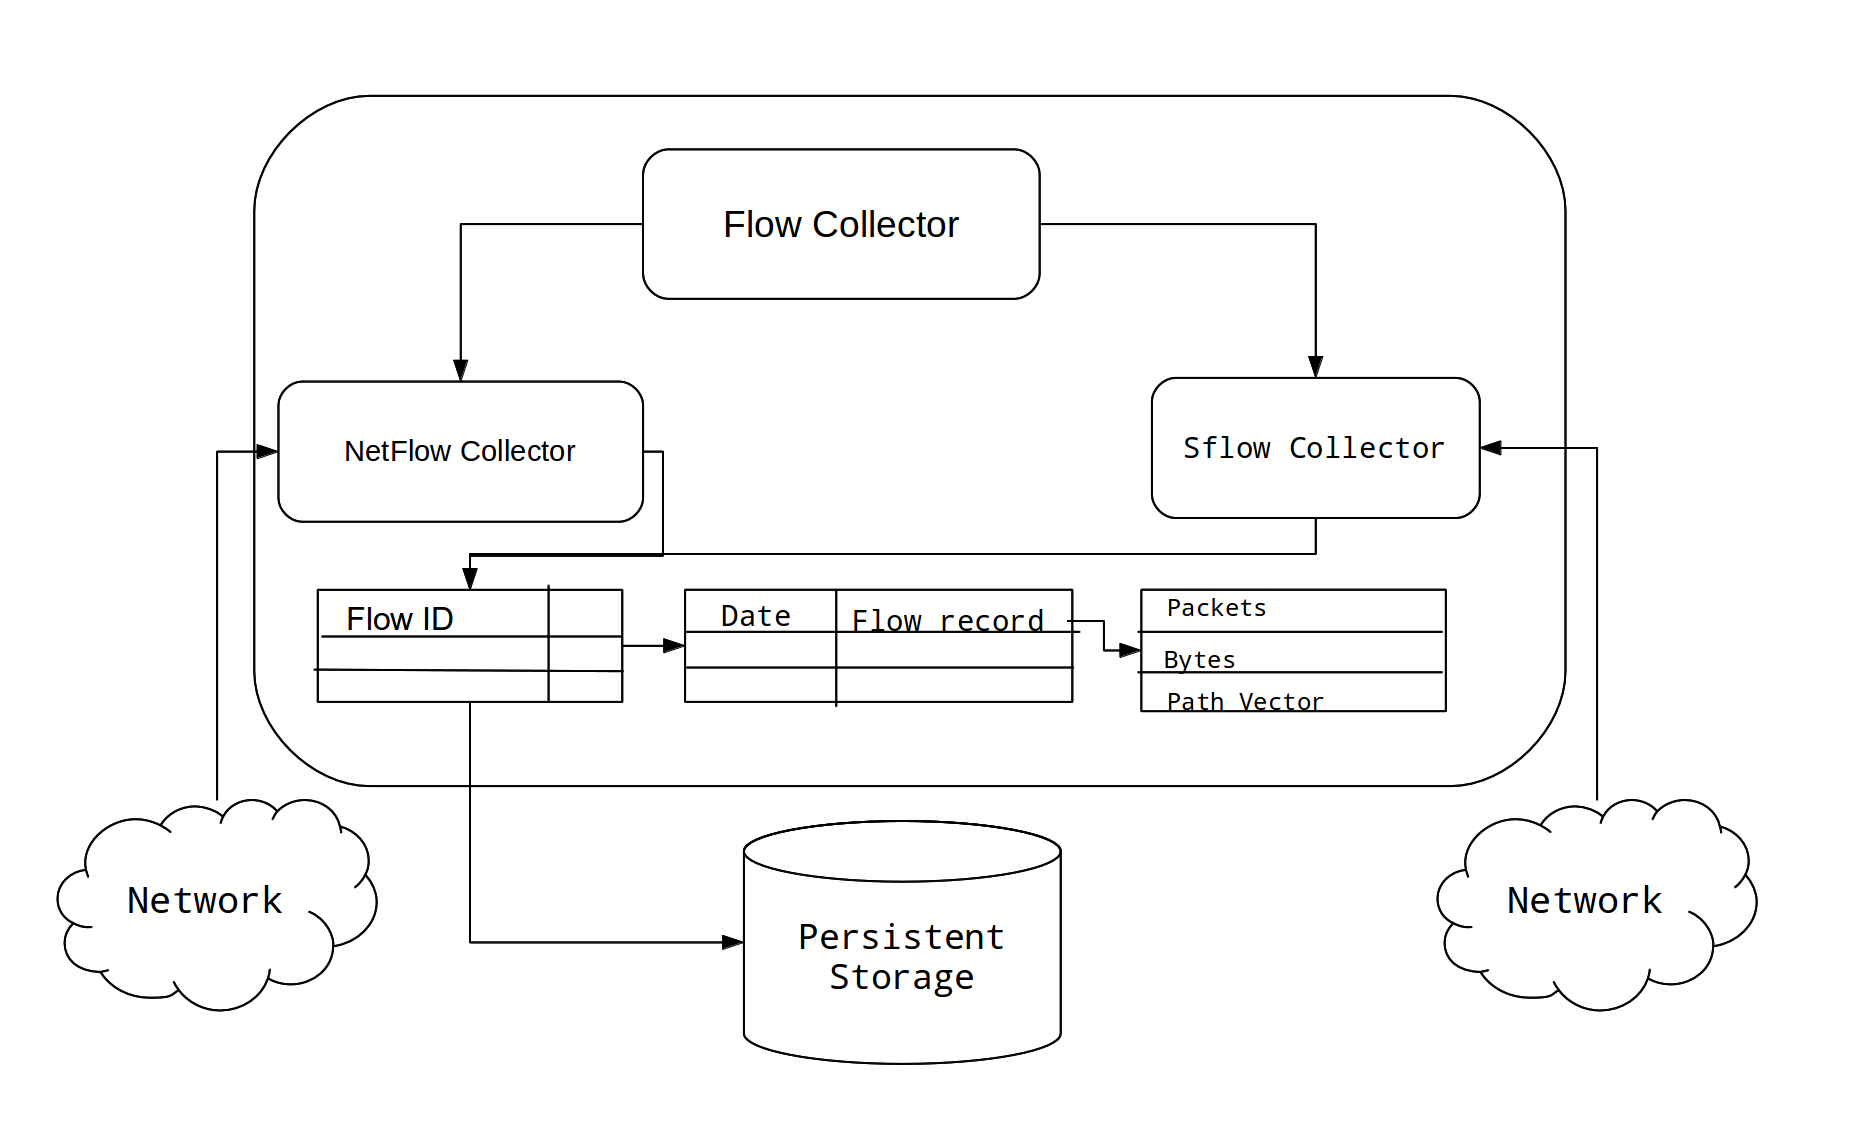
\includegraphics[scale=.35]{emc2.png}
          \caption{Architecture of EMC2.} 
    \end{figure}
    
    Figure 1.1 shows the architecture of EMC2.

    \paragraph\
    EMC2 is a multi-threaded application that contains the following modules:
    \begin{enumerate}
     \item Flow-Table : Flow-Table is an in-memory 2-level hash table.
     \item NetFlowParser : It parses the NetFlow datagrams and updates the Flow-Table.
     %AP: ``It'' is a singular pronoun. Should be associated with a singular verb ``parses'' not the plural verb ``parse''. Similarly ``updates'' and not ``update''. They update, it updates, she updaes, he updates and so on. Please use the proper singular noun/pronoun and verb combinations.
     \item sFlowParser : It parses the sFlow datagrams and updates the Flow-Table.
     %AP: Missing articles: you need to say ``the sFlow'' and ``the Flow-Table'' since you are talking about a specific entity. If you are talking in general, then you need to use the article ``a'' or ``an'' depending on whether the word starts with a consonant or a vowel resp.
     \item NetFlowCollector : It accepts the NetFlow datagrams and creates the parser thread upon receiving NetFlow datagrams.
     \item sFlowCollector : It does the same task like the NetFlowCollector but for sFlow datagrams.
     \item FlowCollector : It invokes two thread -- NetFlowCollector and sFlowCollector -- for accepting flow datagrams.
  \end{enumerate}


    \subsubsection{Flow-Table}
      \paragraph\
	Flow-Table is a 2-level in-memory hash table. The primary key for the hash table is the Flow ID which is formed based on the 
	layer 3 source and destination addresses. Flow ID maps to another hash table where timestamp is the key and flow record is the value. Each flow record contains number of packets, number of bytes and optional path vector.
%AP: Overuse of hyphen (-). Please do not hyphenate everything.

    \subsubsection{NetFlowParser/sFlowParser}
      \paragraph\
	NetFlowCollector and sFlowCollector create these two parser threads upon receiving a NetFlow/sFlow datagram respectively. 
	These parser threads parse the datagram and update the Flow-Table. They also perform two important tasks:
	%AP: ``Parser threads'' is plural - hence use the plural verb ``perform'' not the singular ``performs''. Also, do not keep on saying ``Parser threads''. You can say ``They'' after the first one or two sentences. It is obvious that ``they'' refers to the preceding reference whatever that may be.

	\begin{enumerate}
	 \item Deduplication.
	 \item Data rate prediction in presence of sampling.
	\end{enumerate}
   %AP: Use enumerate wherever possible as it gives you numbering. Bullets are used in more special cases such as primarily in slides etc.
   
   \paragraph{Deduplication:}
       Deduplication prevents duplicate flow records from being added to the Flow-Table. 
       %AP: Please see how I have modified the above sentence from what you had written.
       It uses the following algorithm.
       
       
     \begin{algorithm}[H]
        \caption{Detect Duplicate Flow}
	\label{alg1}

	\begin{algorithmic}
	  \IF{$flow-ID$ not exist}

	      \STATE add flow to the flow table.
	      \RETURN 

	  \ELSE 

	      \IF {Same exporter}
		  \STATE update the flow table.
		  \RETURN 

	      \ELSE

	        \STATE report duplicate flow.
	        \STATE update path vector.
	        \RETURN 

	      \ENDIF

	  \ENDIF

	\end{algorithmic}

       \end{algorithm}

    \paragraph{Data Rate Prediction in Presence of Sampling:}
       Sampling rate is specified in flow datagrams. Parser thread predicts the data rate by multiplying  sampling rate with the length 
       of the packet.
   %AP: This is not clear to me still and as I said does not convey what you told me. I will defer modification of this until I have read the paper.
   
    \subsubsection{NetFlowCollector/sFlowCollector}
      NetFlowCollector/sFlowCollector are collector thread that wait %(AP: wait not waits)
      for new NetFlow or sFlow datagrams and spawn a new NetFlowParser/sFlowParser thread upon receiving a datagram.
      
    \subsection{Advantages and Limitations}
    The authors state the following advantages of EMC2:

    \begin{itemize}
     \item Scalable monitoring as EMC2 monitors host $vswitches$ in a distributed fashion by storing the information as flat files in
     those hosts itself instead of sending them to a centralized collector.
     %AP: I hope the above is correct in terms of the content of the paper.
    \end{itemize}
    
    However, flat files are not really built for scalability unlike many other distributed databases available today such as Cassandra, 
    Big Table etc.. Therefore, it is not clear how much of performance can be obtained by storing the information in flat files in the host 
    itself. Considering that most data centers work with SANs rather than local disks, this may not be as scalable as claimed.
    
    %AP: There is a real problem with your references. But, I will look at how you wrote your .bib file etc. on Monday.

   \section{Scalable Internet Traffic Measurement and Analysis with Hadoop\cite{Lee}}
   \paragraph\
   Hadoop\cite{hadoop} is a distributed computing platform that uses distributed file system(HDFS) and MapReduce\cite{mapreduce} programming model. Hadoop consists of 
   commodity hardware that can scale  thousands of nodes to store massive data. It can perform massive data analytics operations on 
   the available data using MapReduce. Storing NetFlow data on Hadoop and analysis using MapReduce offers scalable traffic 
   measurement and analysis.
   %Nirmoy:add images to describe Hadoop cluster and MapReduce 
    \subsection{Architecture}
     Traffic measurement and analysis system with Hadoop consists of following modules
     \begin{enumerate}
      \item Traffic collector.
      \item IP packet and NetFlow reader in Hadoop.
      \item Analysis in MapReduce.
      \item Interactive query interface with Hive\cite{hive}.
     \end{enumerate}

     \subsubsection{Traffic collector}
     \paragraph\
     Traffic collection done using high-speed packet capture driver and load balancer. Load balancer forwards packets into
     multiple Hadoop DataNodes evenly. Traffic collector also can reads trace files stored on the disk and writes them into HDFS. 
     Trace files contains Netflow packets or IP packets in $libpcap$ format.
     \subsubsection{IP packet and NetFlow reader in Hadoop}
     \paragraph\
      Storing binary trace file into Hadoop specific sequence file needs more computation power as every packet has to be sequentially 
      read from the trace file and stored into HDFS. Authors has develop new Hadoop API to store trace file directly into HDFS. 
      As there is no distinct mark to find out end of a packet records in $libpcap$ format, authors proposed a heuristic algorithm
      using timestamp-based bit pattern.

      \paragraph{MapReduce operation on HDFS to identify packet records:}
	MapReduce job invokes multiple map tasks to process each HDFS block in parallel. Each of the map tasks follow these steps to
	identify packet records in HDFS block:
	\begin{enumerate}
	 \item Read two records using $libpcap$ 16-byte header.
	 \item Check timestamp value, that should be within duration of captured time.
	 \item Wiredlen - caplen $\langle$ maximum packet length.
	 \item Check whether timestamp difference between two packet records within the define threshold threshold. 
	\end{enumerate}
	
	\subsubsection{Analysis in MapReduce}
	Authors has implemented  MapReduce algorithms for processing IP packet as well as NetFlow packets.
	Here is the list of analysis tools
	\begin{enumerate}
	 \item IP Layer analysis provide following analysis job
	      \begin{enumerate}
	       \item Host and port count statistics.
	       \item Periodic flow statistics.
	       \item Periodic sample traffic statistics.
	      \end{enumerate}
	 \item TCP layer analysis compute following statistics
	       \begin{enumerate}
	        \item RTT.
	        \item Retransmission.
	        \item Throughput.
	       \end{enumerate}
	\item NetFlow analysis provides 
	      \begin{enumerate}
	       \item Human readable flow statistics.
	       \item Aggregated flow statistics.
	       \item Top N flows sorted by key such as packet count or byte count. 
	      \end{enumerate}

	\end{enumerate}

      \subsubsection{Interactive query interface with Hive}
      Hive is a data warehousing system build on the top of Hadoop that allows to generate MapReduce jobs using SQl like query.
      IP analysis MapReduce jobs process NetFlow packets on HDFS and  store flow record and IP statistics into
      Hive tables. A user can query on Hive tables using interactive web-based user interface.
      
      \subsection{Advantages and Limitations}
      Advantages of Hadoop based traffic  measurement and analysis are 
	\begin{enumerate}
	  \item Scalable storage.
	  \item MapReduce operations on flow data.
	\end{enumerate}
      Disadvantages of Hadoop based traffic  measurement and analysis are
	\begin{enumerate}
	 \item Low response time- ``the fasted MapReduce job takes 15+ seconds"\cite{mapreducetime}.
	 \item Hadoop NameNode was a single point of failure which solved in later version of 
	        Hadoop 2.0.0 with passive NameNodes.
	 \item Multiple NameNodes require to get high availability\cite{ha}.
	\end{enumerate}
